\chapter{Raspberry Pi mit .Net Core und Blazor}
\label{chp:RaspMitBlazor}
In diesem Kapitel soll ein einfaches Non-Deeply Embedded System mithilfe von Blazor auf einem
Raspberry Pi 4B erstellt werden. Dabei soll gezeigt werden, welche Entwicklungsumgebung genutzt
werden kann und was auf dem Target installiert werden muss.

%sections
\section{Entwicklungsumgebung}
\label{sec:entwicklungsumgebung}
Test
\section{Installation}
\label{sec:installation}
Test

%\section{Programmieren mit .Net Core}
\label{sec:progmitnet}
Test

\section{Blazor Demo Anwendung}
\label{sec:blazordemo}
Nachdem in der letzten Sektion \emph{\nameref{sec:installation}} .Net installiert wurde, soll in
dieser Sektion eine beispielhafte Blazor Anwendung auf dem Raspberry Pi erstellt werden. Die
Anwendung wird auf der \emph{Blazor Server} Architektur basieren. Dabei sollen kontinuierlich
Daten von dem Raspberry Pi abgefragt und auf der Benutzeroberfläche repräsentiert werden.
\subsection{Erstellen des Projektes}
\label{subsec:erstellenProject}
Um eine Blazor Anwendung zu erstellen, gibt es zwei Möglichkeiten. Zum einem vom \emph{Scratch}
aus, aus einer einfachen Konsolen Anwendung, um den notwendigen Code zu implementiert, oder zum
anderen mit hilfe eines Templates. Microsoft bietet einige Templates für verschiedenste
Anwendungen an, die alle samt mit der Installation von .Net kommen.
\newline
\newline
Um nun die Anwendung mithilfe des Templates zu erstellen, muss der folgende Befehl in dem Teminal
eingegeben werden:

\begin{zitat}
    dotnet new blazorserver -o MyApp --no-https
\end{zitat}

Dieser Befehl erstellt eine neue Blazor Server Anwendung, mit dem Namen \emph{MyApp} und
konfiguriert die Anwendung ohne das Https Protokol. Der name sowie, dass kein Https konfiguriert
wird, sind optionale Parameter, die nicht mit angegeben werden müssen. Nachdem die Anwendung 
erfolgreich Installiert wurde, muss noch die Codezeile \emph{webBuilder.UseUrls("Http://*:5000");
} in der \emph{Program.cs} angegeben werden, um die Anwendung für alle Geräte im LAN verfügbar
ist. Der Code in der \emph{Program.cs} sieht dann folgendermaßen aus:

\begin{lstlisting}[language={[Sharp]C}, caption=Program.cs Code,
    label=lst:programCsCode]
    public class Program
    {
        // Main

        public static IHostBuilder CreateHostBuilder(string[] args) =>
            Host.CreateDefaultBuilder(args)
                .ConfigureWebHostDefaults(webBuilder =>
                {
                    webBuilder.UseStartup<Startup>();
                    webBuilder.UseUrls("Http://*:5000"); // <----
                });
    }
\end{lstlisting}

Mit dem Befehl \emph{dotnet run} kann die Anwendung dann gestartet werden. Sobald das Programm
gestartet ist, kann mit dem Link \emph{http://<ip>:5000} die Seite erreicht werden. Sollte alles
geklappt haben sollte nun die Seite, mit den schon vom Template gegebenen Komponenten, wie folgt
angezeigt werden:

\begin{figure}[h]
    \centering
    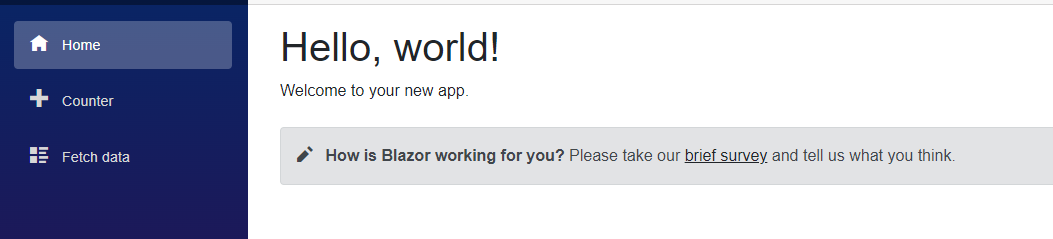
\includegraphics[width=\textwidth, center]{BlazorRasp/ServerTemplate}
    \caption[Blazor Server Template]{Blazor Server Template}
    \label{img:BlazorServerTemplate}
\end{figure}
\subsection{Microsoft IoT}
\label{subsec:MicrosoftIot}
Damit mit dem Raspberry Pi kommuniziert werden kann, können Bibliotheken verwendet werden.
Microsoft bietet eine IoT Bibliothek an, mit der die Sensoren oder die LEDs auf
dem Gerät angesteuert werden können. Die Bibliothek kann wie folgt in das Projekt eingebunden
werden:

\begin{lstlisting}[language={[Sharp]C}, caption=IoT NuGet Package,
    label=lst:IotNugetPackage]
    <ItemGroup>
    <PackageReference Include="Iot.Device.Bindings" Version="1.5.0-*" />
  </ItemGroup>
\end{lstlisting}

Das folgende beispielhafte Konsolenprogramm demonstriert, wie auf die Daten zugegriffen werden kann:

\begin{lstlisting}[language={[Sharp]C}, caption=SenseHat Beispielprogramm,
    label=lst:SenseHatBeispielProgramm]
    public class Program
    {
        static void Main(string[] args)
        {
            using SenseHat _senseHat = new();

            Console.WriteLine($"Temperatur: {_senseHat.Temperature.DegreesCelsius:0.#}\u00B0C");
            Console.WriteLine($"Temperatur 2: {_senseHat.Temperature2.DegreesCelsius:0.#}\u00B0C");
            Console.WriteLine($"Luftdruck: {_senseHat.Pressure.Hectopascals:0.##} hPa");
            Console.WriteLine($"Luftfeuchtigkeit: {_senseHat.Humidity.Percent:0.#}%");
        }
    }
\end{lstlisting}

Der Output durch obiges Programm sieht wie folgt aus:

\begin{zitat}
    Temperatur: 38,4°C
    \newline
    Temperatur 2: 38,5°C
    \newline
    Luftdruck: 984,03 hPa
    \newline
    Luftfeuchtigkeit: 31\%
\end{zitat}
\subsection{Raspberry Pi Daten Anzeigen}
\label{subsec:DatenAnzeigen}
In dieser Sektion soll nun die Logik implementiert werden, um die Daten, die vom Raspberry Pi
kommen, auf der Benutzeroberfläche anzuzeigen. Dafür wird ein \emph{Timer} implementiert werden, der
jede Sekunde auslöst, um dann die Daten zu lesen.
\newline
\newline
Damit etwas auf der Benutzeroberfläche angezeigt werden kann, muss das \emph{Html-Markup}
implementiert werden:

\begin{lstlisting}[language={[Sharp]C}, caption=Html-Markup,
    label=lst:HtmlMarkup]
<div class="divHeader">
    <div>
        <h1>Raspberry Pi</h1>

        <h2>Uhrzeit: @_uhrzeit</h2>
    </div>

    <div>
        <h3>Temperature Sensor 1: @_temperatur</h3>
        <h3>Temperature Sensor 2: @_temperatur2</h3>
        <h3>Luftdruck: @_pressure</h3>
        <h3>Luftfeuchtigkeit: @_humidity</h3>
    </div>
</div>
\end{lstlisting}

Dabei signalisiert das \emph{@<name>}, dass es sich dabei um eine Variable handelt, die im Code
deklariert wurde.
\newline
\newline
Weitergehend bietet Blazor verschiedene \emph{Render-Funktionen} die nach bestimmten ereignissen
aufgerufen werden. Wie zum Beispiel die \emph{OnInitializedAsync}, die aufgerufen wird, wenn die
Komponente geladen wird. Diese \emph{OnInitializedAsync} kann nun dazu gebraucht werden, um die
Variablen zu initialisieren.

\begin{lstlisting}[language={[Sharp]C}, caption=Render-Funktion: OnInitializedAsync,
    label=lst:OnInitializedAsync]
    protected override Task OnInitializedAsync()
    {
        _senseHat = new();
        _cultureInfo = new("de-DE");
        _uhrzeit = DateTime.Now.ToString("HH:mm:ss", _cultureInfo);

        _temperatur = string.Empty;
        _temperatur2 = string.Empty;
        _pressure = string.Empty;
        _humidity = string.Empty;

        return base.OnInitializedAsync();
    }
\end{lstlisting}

Nun soll zudem noch eine Hilfsfunktion \emph{SetRaspValues} geschaffen werden, die die Daten
ausliest. Diese Funktion wird dann auch in der \emph{OnInitializedAsync} Funktion aufgerufen.

\begin{lstlisting}[language={[Sharp]C}, caption=Funktion: SetRaspValues,
    label=lst:SetRaspValues]
    private void SetRaspValues()
    {
        _temperatur = $"{_senseHat.Temperature.DegreesCelsius:0.#}\u00B0C";
        _temperatur2 = $"{_senseHat.Temperature2.DegreesCelsius:0.#}\u00B0C";
        _pressure = $"{_senseHat.Pressure.Hectopascals:0.##} hPa";
        _humidity = $"{_senseHat.Humidity.Percent:0.#}%";
    }
\end{lstlisting}

Damit die Daten jedoch nicht nur einmal am Anfang gelesen werden, sondern sich kontinuierlich
aktuallisieren, soll ein \emph{Timer} jede Sekunde getriggert werden, um die Daten neu zu lesen
und dem \emph{DOM} mitzuteilen, dass sich der \emph{State} der Seite geändert hat.

\begin{lstlisting}[language={[Sharp]C}, caption=Timer: ReadTimer,
    label=lst:ReadTimer]
    private void StartTimer()
    {
        _readTimer = new(1000);
        _readTimer.Elapsed += GetData;
        _readTimer.Enabled = true;
    }

    private void GetData(Object source, System.Timers.ElapsedEventArgs e)
    {
        _uhrzeit = DateTime.Now.ToString("HH:mm:ss", cultureInfo);
        SetRaspValues();
        InvokeAsync(StateHasChanged);
    }
\end{lstlisting}

Wichtig hierbei ist jedoch, dass die Funktion \emph{StateHasChanged} manuell aufgerufen
wurde. Dies übernimmt Blazor normalerweise schon automatisch, wenn sich Variablen der Komponente
verändern, die angezeigt werden aber da hier die Variablen nicht auf dem \emph{Ui-Thread} geändert
wurden, muss manuell angegeben werden, dass sich der \emph{State} geändert hat.
\newline
\newline
Der momentane Stand der Seite zieht so aus:

\begin{figure}[h]
    \centering
    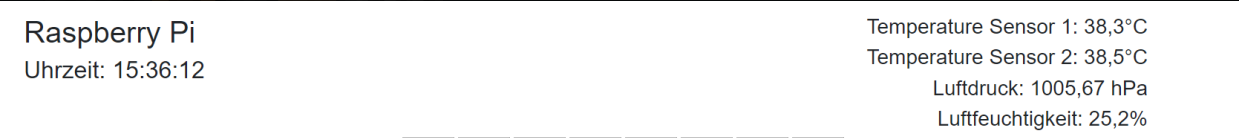
\includegraphics[width=\textwidth, center]{BlazorRasp/BlazorDatenAnzeigen}
    \caption[Zwischenstand der Blazor Demo]{Zwischenstand der Blazor Demo}
    \label{img:BlazorDatenAnzeigen}
\end{figure}
\subsection{LED-Matrix ansteuern}
\label{subsec:ledMatrix}
In dieser Sektion soll eine \emph{8x8 Button-Matrix} erstellt werden, die die \emph{8x8
LED-Matrix} auf dem Sensehat des Raspberry Pi repräsentieren soll. Dabei soll der vorhandene
Joystick auf dem Sensehat genutzt werden, um über die Button-Matrix zu navigieren und die
LEDs zu platzieren.
\newline
\newline
Da Blazor die \emph{Razor-Syntax} verwendet, kann jegliche C\# Kontrollstruktur im
\emph{HTML-Markup} verwendet werden. So kann dies wie folgt genutzt werden, um die \emph{8x8
Button-Matrix} zu erzeugen:

\begin{lstlisting}[language={[Sharp]C}, caption=Button-Matrix,
    label=lst:ButtonMatrix]
<div class="divGrid">
    @for (var y = 0; y < LengthY; y++)
    {
        @for (var x = 0; x < LengthX; x++)
        {
            int copyY = y;
            int copyX = x;
            <Button class="buttonBox @classes[copyY,copyX]"/>
        }
    }
</div>
\end{lstlisting}

Das \emph{@classes} Element ist ein Zwei-Dimensionales Array aus Strings, mit der
CSS-Klassen hinzugefügt und wieder gelöscht werden sollen. Um zu ermitteln, welcher
Joystick-Button betätigt wurde, soll ein weiterer
\emph{Timer} zum Einsatz kommen. Dieser Timer soll alle 15 Millisekunden ausgelöst werden.

\begin{lstlisting}[language={[Sharp]C}, caption=Timer: _setButtonTimer,
    label=lst:ButtonTimer]
    private void StartTimer()
    {
        // More Code

        _setButtonTimer = new(15);
        _setButtonTimer.Elapsed += WriteStateToChannel;
        _setButtonTimer.Enabled = true;
    }


    private async void WriteStateToChannel(Object source, System.Timers.ElapsedEventArgs e)
    {
        if((ticks - lastTicks) > 9){
            _senseHat.ReadJoystickState();
            if(_senseHat.HoldingButton){
                await _stateChannel.Writer.WriteAsync(JoystickState.Holding);
            }
            else if(_senseHat.HoldingUp){
                await _stateChannel.Writer.WriteAsync(JoystickState.Up);
            }
            else if(_senseHat.HoldingDown){
                await _stateChannel.Writer.WriteAsync(JoystickState.Down);
            }
            else if(_senseHat.HoldingLeft){
                await _stateChannel.Writer.WriteAsync(JoystickState.Left);
            }
            else if(_senseHat.HoldingRight){
                await _stateChannel.Writer.WriteAsync(JoystickState.Right);
            }
            lastTicks = ticks;
        }
        ticks++;
    }
\end{lstlisting}

Bei \emph{JoystickState} handelt es sich um ein Enum, welches den \emph{State} des Joysticks
repräsentieren soll. Wie zu sehen ist, wird der aktuelle \emph{State} des Joysticks gelesen, um
das Ergebnis in einen \emph{Channel} zu schreiben.
\newline
\newline
Für die Verarbeitung des \emph{States}, wird in \emph{OnInitializedAsync} ein Task gestartet, der
in einer Endlosschleife läuft und darauf warte bis etwas in den \emph{Channel} hinzugefügt
wird. Sobald sich der \emph{State} geändert hat, wird entweder die Position berechnet oder
die LED an dieser Position leuchtet in einer neuen Farbe.

\begin{lstlisting}[language={[Sharp]C}, caption=Task zum Verarbeiten des States,
    label=lst:StateTask]
        _setButtonTask = Task.Run(async () =>
        {
            while (true)
            {
                if(cancellationToken.IsCancellationRequested)
                    cancellationToken.ThrowIfCancellationRequested();
                var state = await _stateChannel.Reader.ReadAsync();
                int x = 0;
                int y = 0;
                if(state == JoystickState.Holding){
                    SetButtonBackground(_currentX, _currentY);
                }
                else if(state == JoystickState.Up){
                    y--;
                }
                else if(state == JoystickState.Down){
                    y++;
                }
                else if(state == JoystickState.Left){
                    x--;
                }else if(state == JoystickState.Right){
                    x++;
                }
                SetPositions(x, y);
                RemoveButtonBorder(_previousX, _previousY);
                SetButtonBorder(_currentX, _currentY);
                await InvokeAsync(StateHasChanged);
            }
        });

    private void SetButtonBackground(int x, int y)
    {
        if (classes[y, x].Contains(" setBackground"))
        {
            _senseHat.SetPixel(x, y, Color.Blue);
            classes[y, x] = classes[y, x].Replace(" setBackground", string.Empty);
        }
        else
        {
            _senseHat.SetPixel(x, y, Color.Red);
            classes[y, x] += " setBackground";
        }
    }
\end{lstlisting}

Wie zu erkennen ist, wird die LED und der Button je
nach vorherigem Zustand entweder Blau oder Rot. Die entstandene Anwendung sieht dann wie folgt aus:

\begin{figure}[h]
    \centering
    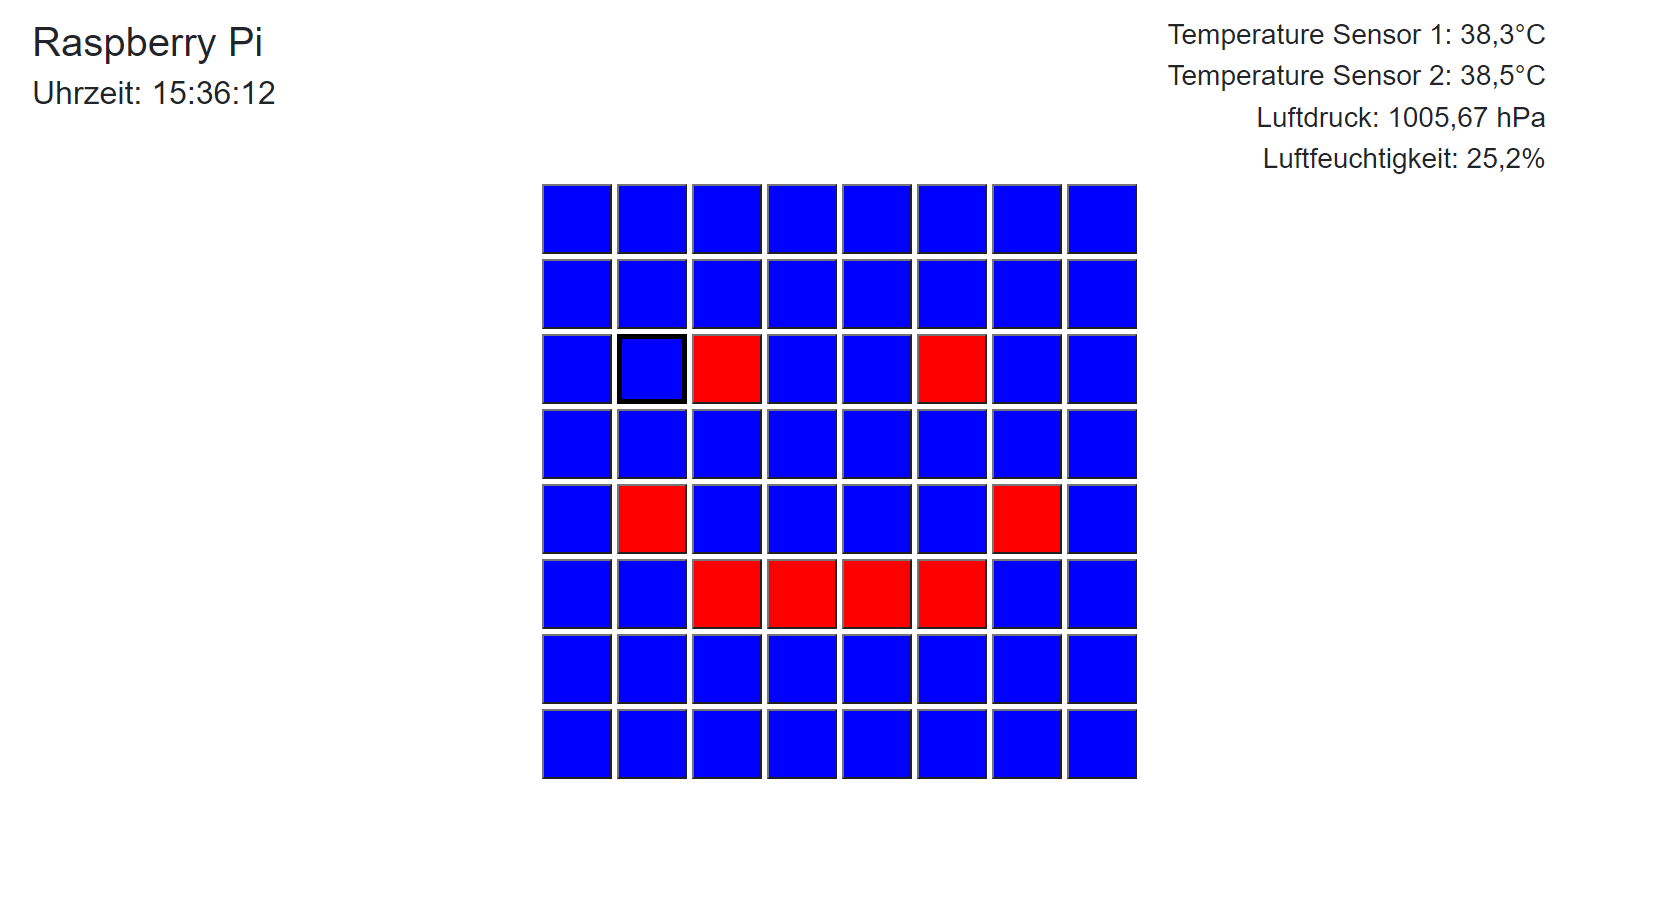
\includegraphics[width=\textwidth, center]{BlazorRasp/Demo}
    \caption[Blazor Demo]{Blazor Demo}
    \label{img:BlazorDatenAnzeigen}
\end{figure}

Da nur technisch relevante Code Abschnitte in diesem Kapitel präsentiert wurden, ist der
komplette Code im Anhang \ref{lst:DemoCode} zu finden.